\documentclass[english, 11 pt, class=article, crop=false]{standalone}
\usepackage[T1]{fontenc}
%\renewcommand*\familydefault{\sfdefault} % For dyslexia-friendly text
\usepackage{lmodern} % load a font with all the characters
\usepackage{geometry}
\geometry{verbose,paperwidth=16.1 cm, paperheight=24 cm, inner=2.3cm, outer=1.8 cm, bmargin=2cm, tmargin=1.8cm}
\setlength{\parindent}{0bp}
\usepackage{import}
\usepackage[subpreambles=false]{standalone}
\usepackage{amsmath}
\usepackage{amssymb}
\usepackage{esint}
\usepackage{babel}
\usepackage{tabu}
\makeatother
\makeatletter

\usepackage{titlesec}
\usepackage{ragged2e}
\RaggedRight
\raggedbottom
\frenchspacing

% Norwegian names of figures, chapters, parts and content
\addto\captionsenglish{\renewcommand{\figurename}{Figur}}
\makeatletter
\addto\captionsenglish{\renewcommand{\chaptername}{Kapittel}}
\addto\captionsenglish{\renewcommand{\partname}{Del}}


\usepackage{graphicx}
\usepackage{float}
\usepackage{subfig}
\usepackage{placeins}
\usepackage{cancel}
\usepackage{framed}
\usepackage{wrapfig}
\usepackage[subfigure]{tocloft}
\usepackage[font=footnotesize,labelfont=sl]{caption} % Figure caption
\usepackage{bm}
\usepackage[dvipsnames, table]{xcolor}
\definecolor{shadecolor}{rgb}{0.105469, 0.613281, 1}
\colorlet{shadecolor}{Emerald!15} 
\usepackage{icomma}
\makeatother
\usepackage[many]{tcolorbox}
\usepackage{multicol}
\usepackage{stackengine}

\usepackage{esvect} %For vectors with capital letters

% For tabular
\usepackage{array}
\usepackage{multirow}
\usepackage{longtable} %breakable table

% Ligningsreferanser
\usepackage{mathtools}
\mathtoolsset{showonlyrefs}

% index
\usepackage{imakeidx}
\makeindex[title=Indeks]

%Footnote:
\usepackage[bottom, hang, flushmargin]{footmisc}
\usepackage{perpage} 
\MakePerPage{footnote}
\addtolength{\footnotesep}{2mm}
\renewcommand{\thefootnote}{\arabic{footnote}}
\renewcommand\footnoterule{\rule{\linewidth}{0.4pt}}
\renewcommand{\thempfootnote}{\arabic{mpfootnote}}

%colors
\definecolor{c1}{cmyk}{0,0.5,1,0}
\definecolor{c2}{cmyk}{1,0.25,1,0}
\definecolor{n3}{cmyk}{1,0.,1,0}
\definecolor{neg}{cmyk}{1,0.,0.,0}

% Lister med bokstavar
\usepackage[inline]{enumitem}

\newcounter{rg}
\numberwithin{rg}{chapter}
\newcommand{\reg}[2][]{\begin{tcolorbox}[boxrule=0.3 mm,arc=0mm,colback=blue!3] {\refstepcounter{rg}\phantomsection \large \textbf{\therg \;#1} \vspace{5 pt}}\newline #2  \end{tcolorbox}\vspace{-5pt}}

\newcommand\alg[1]{\begin{align} #1 \end{align}}

\newcommand\eks[2][]{\begin{tcolorbox}[boxrule=0.3 mm,arc=0mm,enhanced jigsaw,breakable,colback=green!3] {\large \textbf{Eksempel #1} \vspace{5 pt}\\} #2 \end{tcolorbox}\vspace{-5pt} }

\newcommand{\st}[1]{\begin{tcolorbox}[boxrule=0.0 mm,arc=0mm,enhanced jigsaw,breakable,colback=yellow!12]{ #1} \end{tcolorbox}}

\newcommand{\spr}[1]{\begin{tcolorbox}[boxrule=0.3 mm,arc=0mm,enhanced jigsaw,breakable,colback=yellow!7] {\large \textbf{Språkboksen} \vspace{5 pt}\\} #1 \end{tcolorbox}\vspace{-5pt} }

\newcommand{\sym}[1]{\colorbox{blue!15}{#1}}

\newcommand{\info}[2]{\begin{tcolorbox}[boxrule=0.3 mm,arc=0mm,enhanced jigsaw,breakable,colback=cyan!6] {\large \textbf{#1} \vspace{5 pt}\\} #2 \end{tcolorbox}\vspace{-5pt} }

\newcommand\algv[1]{\vspace{-11 pt}\begin{align*} #1 \end{align*}}

\newcommand{\regv}{\vspace{5pt}}
\newcommand{\mer}{\textsl{Merk}: }
\newcommand{\mers}[1]{{\footnotesize \mer #1}}
\newcommand\vsk{\vspace{11pt}}
\newcommand\vs{\vspace{-11pt}}
\newcommand\vsb{\vspace{-16pt}}
\newcommand\sv{\vsk \textbf{Svar} \vspace{4 pt}\\}
\newcommand\br{\\[5 pt]}
\newcommand{\figp}[1]{../fig/#1}
\newcommand\algvv[1]{\vs\vs\begin{align*} #1 \end{align*}}
\newcommand{\y}[1]{$ {#1} $}
\newcommand{\os}{\\[5 pt]}
\newcommand{\prbxl}[2]{
\parbox[l][][l]{#1\linewidth}{#2
	}}
\newcommand{\prbxr}[2]{\parbox[r][][l]{#1\linewidth}{
		\setlength{\abovedisplayskip}{5pt}
		\setlength{\belowdisplayskip}{5pt}	
		\setlength{\abovedisplayshortskip}{0pt}
		\setlength{\belowdisplayshortskip}{0pt} 
		\begin{shaded}
			\footnotesize	#2 \end{shaded}}}

\renewcommand{\cfttoctitlefont}{\Large\bfseries}
\setlength{\cftaftertoctitleskip}{0 pt}
\setlength{\cftbeforetoctitleskip}{0 pt}

\newcommand{\bs}{\\[3pt]}
\newcommand{\vn}{\\[6pt]}
\newcommand{\fig}[1]{\begin{figure}
		\centering
		\includegraphics[]{\figp{#1}}
\end{figure}}

\newcommand{\figc}[2]{\begin{figure}
		\centering
		\includegraphics[]{\figp{#1}}
		\caption{#2}
\end{figure}}

\newcommand{\sectionbreak}{\clearpage} % New page on each section

\newcommand{\nn}[1]{
\begin{equation}
	#1
\end{equation}
}

% Equation comments
\newcommand{\cm}[1]{\llap{\color{blue} #1}}

\newcommand\fork[2]{\begin{tcolorbox}[boxrule=0.3 mm,arc=0mm,enhanced jigsaw,breakable,colback=yellow!7] {\large \textbf{#1 (forklaring)} \vspace{5 pt}\\} #2 \end{tcolorbox}\vspace{-5pt} }
 
%colors
\newcommand{\colr}[1]{{\color{red} #1}}
\newcommand{\colb}[1]{{\color{blue} #1}}
\newcommand{\colo}[1]{{\color{orange} #1}}
\newcommand{\colc}[1]{{\color{cyan} #1}}
\definecolor{projectgreen}{cmyk}{100,0,100,0}
\newcommand{\colg}[1]{{\color{projectgreen} #1}}

% Methods
\newcommand{\metode}[2]{
	\textsl{#1} \\[-8pt]
	\rule{#2}{0.75pt}
}

%Opg
\newcommand{\abc}[1]{
	\begin{enumerate}[label=\alph*),leftmargin=18pt]
		#1
	\end{enumerate}
}
\newcommand{\abcs}[2]{
	\begin{enumerate}[label=\alph*),start=#1,leftmargin=18pt]
		#2
	\end{enumerate}
}
\newcommand{\abcn}[1]{
	\begin{enumerate}[label=\arabic*),leftmargin=18pt]
		#1
	\end{enumerate}
}
\newcommand{\abch}[1]{
	\hspace{-2pt}	\begin{enumerate*}[label=\alph*), itemjoin=\hspace{1cm}]
		#1
	\end{enumerate*}
}
\newcommand{\abchs}[2]{
	\hspace{-2pt}	\begin{enumerate*}[label=\alph*), itemjoin=\hspace{1cm}, start=#1]
		#2
	\end{enumerate*}
}

% Oppgaver
\newcommand{\opgt}{\phantomsection \addcontentsline{toc}{section}{Oppgaver} \section*{Oppgaver for kapittel \thechapter}\vs \setcounter{section}{1}}
\newcounter{opg}
\numberwithin{opg}{section}
\newcommand{\op}[1]{\vspace{15pt} \refstepcounter{opg}\large \textbf{\color{blue}\theopg} \vspace{2 pt} \label{#1} \\}
\newcommand{\ekspop}[1]{\vsk\textbf{Gruble \thechapter.#1}\vspace{2 pt} \\}
\newcommand{\nes}{\stepcounter{section}
	\setcounter{opg}{0}}
\newcommand{\opr}[1]{\vspace{3pt}\textbf{\ref{#1}}}
\newcommand{\oeks}[1]{\begin{tcolorbox}[boxrule=0.3 mm,arc=0mm,colback=white]
		\textit{Eksempel: } #1	  
\end{tcolorbox}}
\newcommand\opgeks[2][]{\begin{tcolorbox}[boxrule=0.1 mm,arc=0mm,enhanced jigsaw,breakable,colback=white] {\footnotesize \textbf{Eksempel #1} \\} \footnotesize #2 \end{tcolorbox}\vspace{-5pt} }
\newcommand{\rknut}{
Rekn ut.
}

%License
\newcommand{\lic}{\textit{Matematikken sine byggesteinar by Sindre Sogge Heggen is licensed under CC BY-NC-SA 4.0. To view a copy of this license, visit\\ 
		\net{http://creativecommons.org/licenses/by-nc-sa/4.0/}{http://creativecommons.org/licenses/by-nc-sa/4.0/}}}

%referances
\newcommand{\net}[2]{{\color{blue}\href{#1}{#2}}}
\newcommand{\hrs}[2]{\hyperref[#1]{\color{blue}\textsl{#2 \ref*{#1}}}}
\newcommand{\rref}[1]{\hrs{#1}{regel}}
\newcommand{\refkap}[1]{\hrs{#1}{kapittel}}
\newcommand{\refsec}[1]{\hrs{#1}{seksjon}}

\newcommand{\mb}{\net{https://sindrsh.github.io/FirstPrinciplesOfMath/}{MB}}


%line to seperate examples
\newcommand{\linje}{\rule{\linewidth}{1pt} }

\usepackage{datetime2}
%%\usepackage{sansmathfonts} for dyslexia-friendly math
\usepackage[]{hyperref}

%\usepackage{xr}
%\externaldocument{/home/sindre/P/bok1P_pdf}
\geometry{a4paper,verbose,tmargin=1cm,bmargin=2cm,lmargin=4cm,rmargin=4cm,headheight=3cm,headsep=1cm,footskip=1cm}
\newcounter{inl}
\newcounter{abc}
%\numberwithin{inl}{}
\newcommand{\inl}[1]{\vspace{15pt} \setcounter{abc}{0} \refstepcounter{inl} {\Large \textbf{Oppgave \theinl\;\textendash\,#1}} \vspace{5 pt}\\}
\renewcommand\theabc{\alph{abc}}
\newcommand{\ab}{\refstepcounter{abc} \textbf{\theabc}) }
\begin{document}
\theabc
{\huge Innlevering 2: Repetisjon av kapittel 1-7}\vsk
\begin{itemize}
	\item Innleveringen blir vurdert med karakter.
	\item For å bestå innleveringen (oppnå karakteren 2) må \textsl{minimum} hele \textsl{Oppgave 1} være gjort.	
	\item Hele \textsl{Oppgave 1} skal føres for hand. I de andre oppgavene er det oppgitt hvilke oppgaver som må føres for hand.
	\item Under alle handskrevne svar skal du har to linjalstreker under.
	\item Samarbeid er lov, men skriv på arket hvem du har samarbeidet med.
	\item I vurderingen av \textsl{Oppgave 2} og \textsl{3} blir det lagt stor vekt på hvor flink du er til å forklare utregningene du gjør. Gode hjelpetegninger vil telle positivt, men er ikke nødvendig for å oppnå høyeste karakter.


\end{itemize}
\newpage

\inl{Regning for hand}
\ab
Regn ut og vis utregning (sjekk gjerne videoene du finner i modulen \net{https://akademiet.instructure.com/courses/5115}{\textsl{Tips og triks}}):\os
\begin{tabular}{@{}l l l l}
	II) $ 12,7\cdot 4 $&
	II) $ 2,4\cdot 3,5 $&
	III) ${ 100:8} $\br
\end{tabular}\vsk


\ab
Gjør om:\os
\begin{tabular}{@{}l l l l}
	I) 15\,kg målt i g.&
	II) 2\,400\,m målt i mil.\br
	III) 174\,m$ ^2 $ målt i km$ ^2 $.	&
	IV) 0,000023\,km$ ^3 $ målt i L.
\end{tabular}\vsk

\ab Gjør disse oppgavene fra boka: 3.1.1ab, 3.2.1b, 3.2.2, 3.4.1b, 4.2.1b, 4.3.1b

\inl{Veikonstruktøren}
Du har fått i oppgave å konstruere en bilbro over én av Norges mange fjorder. På den éne siden av broen er det en bratt bakke, mens på den andre er det to kraftige svinger, så broprosjektet avhenger av at du gjør noen treffsikre beregninger. \vsk

\prbxl{0.6}{\ab Når en bakke er veldig bratt må man sette opp et skilt som varsler om dette, et slikt skilt skal informere om stigningen i prosent. Denne prosenten blir regnet ut slik:\os
	\textsl{Man finner først ut hvor høyt man stiger per meter man beveger seg bortover. Så finner man ut hvor mange prosent høyden ugtjør av lengden bortover.}
}\qquad
\parbox[r][][l]{0.3\linewidth}{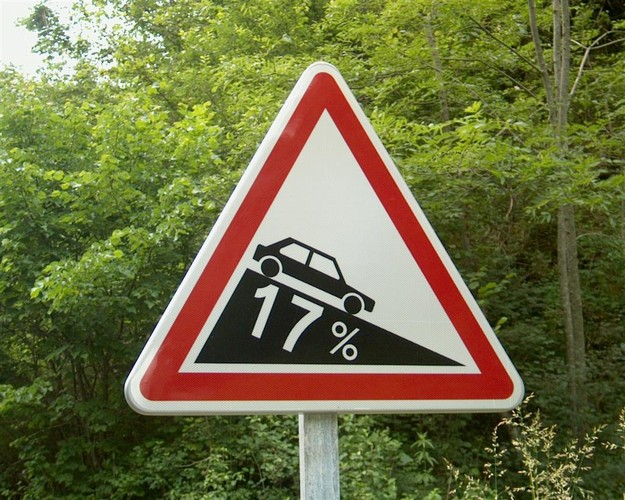
\includegraphics[scale=0.15]{stign}\\ \vspace{8pt}
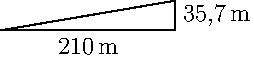
\includegraphics[scale=0.8]{fig/bakke}
}\vspace{8pt}
\textsl{Eksempel: Hvis man stiger 35,7\,m når man har kjørt 210 m rett bort, er stigningen $ {\frac{35,7}{210}=0,17=17\%} $}.\os

Etter å ha kjørt over broen vestover, kommer bilistene inn i en bakke der man stiger 64\,m på 800\,m rett bort. Hvilken stigning må stå på skiltet du må sette opp for denne bakken? (\textsl{Denne oppgaven skal gjøres for hand}).\vsk

\ab De nevnte svingene studerer vi på et kart som har målestokken $ 1:2000 $. Den minste svingen har en radius på 3\,cm, mens den største svingen har en radius på 6\,cm. Videre vet vi også at $ {AS=6\enh{cm}} $ og $ {SC=12\enh{cm}} $ mellom sentrum til svingene. For å hjelpe oss i planleggingen lager vi figuren under:
\begin{figure}
	\centering
	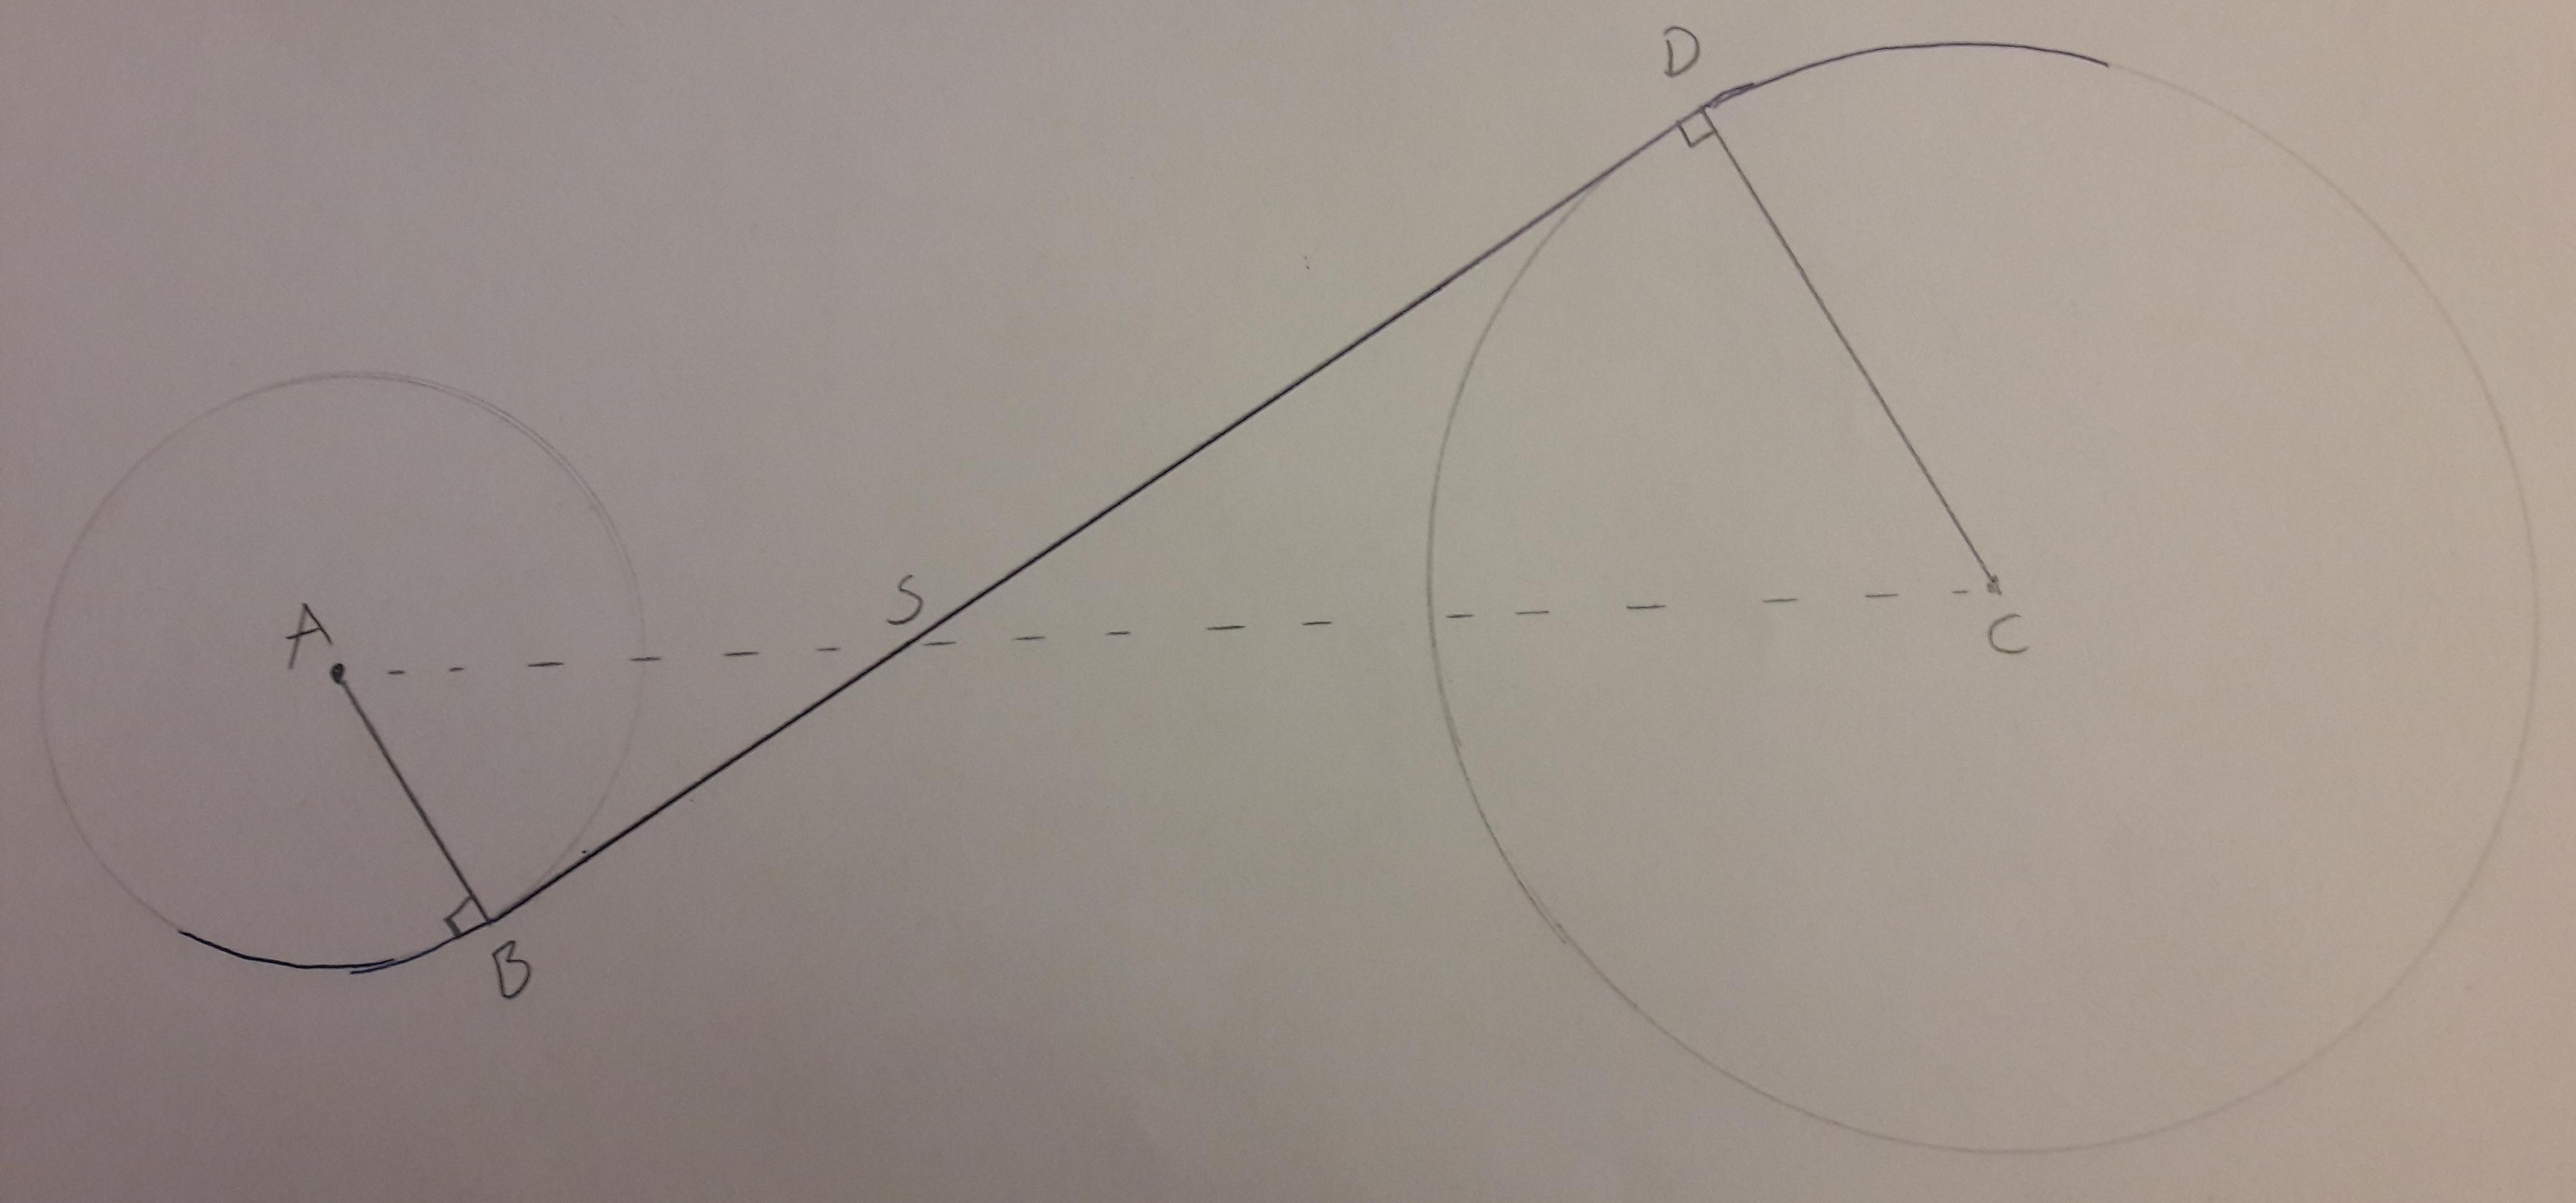
\includegraphics[scale=0.07]{fig/vei}
\end{figure}
Forklar hvorfor trekantene $ \triangle ABS $ og $ \triangle SCD $ er formlike. \os
I) Finn de samsvarende sidene i trekantene.\os

II) Finn hvor lang den rette strekningen mellom svingene er i virkeligheten.\os

\ab Broen skal stå på sylinderformede pilarer (søyler) som på det høyeste er 30\,m, og som har radius 2 m. Pilarene skal støpes i betong. Hvor mange liter betong trenger du for hver av de høyeste pilarene? (\textsl{Regn ut svaret for hånd, hvor du bruker $ {\pi\approx3} $, og med kalkulator, hvor du bruker $ {\pi\approx3,14} $}.)\vsk

\ab Betong er en blanding av sement, sand, stein og ferskvann. \net{http://bmc-norge.no/index.php?option=com_content&view=category&layout=blog&id=98&Itemid=495}{BMC} opplyser at for å få 1$ \,\enh{m}^3 $ med betong må du blande følgende:\\ \begin{figure}
	\centering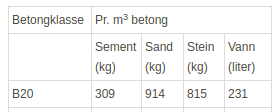
\includegraphics[scale=0.6]{fig/betong}
\end{figure}
I) Hva er forholdet mellom antall kg sement+sand+stein og antall liter vann?\os
II) Hvor mye sement, sand og stein må du til sammen ha for å lage nok sement til den høyeste pilaren? \os

III) For å være på den sikre siden bruker du til sammen 978\,240 kg med sement+sand+stein. Hvor mye vann må du da fylle i blandingen?

\inl{Bakeren}

(\textsl{Obs!} Oppgave b)  er ganske vanskelig. Hvis du ikke greier å løse oppgavene du finner der, kan du bruke tallene fra fasiten for å løse oppgavene som kommer etterpå.)\vsk

Du har blitt utnevnt til Hans Majestet Kongens Baker, og i den anledning skal du bake et pepperkakehus formet som slottet. Slottet skal bakes i måle-\\stokken $ {1:500} $.
Se \net{http://www.kongehuset.no/artikkel.html?tid=27631&sek=27447}{her} og \net{https://www.google.no/maps/place/The+Royal+Palace/@59.9172048,10.7263948,155m/data=!3m1!1e3!4m5!3m4!1s0x0:0x677038c9acc2591c!8m2!3d59.9170428!4d10.7273769}{her} for info om slottet.\vsk

\ab Tegn slottet i oppgitt målestokk på et millimeterpapir. (Vis utregningen for hvordan du fant de forskjellig lengdene du tegner inn). \vsk

\ab Du tar utgangspunkt i oppskriften til
\net{https://www.nrk.no/mat/pepperkaker-og-pepperkakehus-1.7123944}{nrk}, der står det at veggene skal være 0,5\,cm tykke.\os

I) Beregn hvor mye (i liter) deig du trenger for å lage veggene på pepperkakehuset ditt.\os

II) Beregn hvor mye (i liter) deig du trenger for å lage taket på pepperkakehuset ditt.\os

\textsl{Obs!} For å løse oppgave II) kan du trenge dette:  
På figuren under ser du en skisse av takkonstruksjonen til slottet. 
\begin{figure}
	\centering
	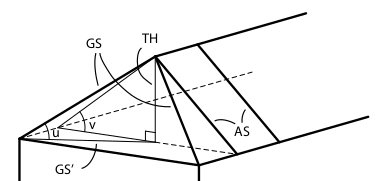
\includegraphics[scale=0.6]{valt}\quad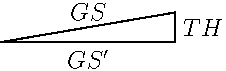
\includegraphics[scale=1]{fig/gs}
\end{figure}
Bruk den rettvinklete trekanten dannet av sidene $ TH $, $ GS' $ og $ GS $ til å finne $ GS $ når du vet at $ {TH=6,15\enh{m}} $ og $ {GS'=17,05\enh{m}} $.\os 
Videre vil du ha nytte av å vite at  $ {AS = 13,52\enh{m}} $ og at toppen av taket er ca 76\,m langt for å beregne de to største takplatene. Takene til sidefløyene kan du regne som to flate firkanter.\vsk
 
\ab Istedenfor metoden du brukte i forrige oppgave, bruker arkitektene en formel for å finne lengden av $ GS $. I dette tilfellet er $ GS $ gitt ved formelen:
\[ GS = \frac{b \sqrt{2}\cdot50}{47} \]
hvor $ b $ er halve bredden til hovedfløyen.
Bruk formelen til å sjekke at du har funnet riktig lengde av $ GS $. \vsk
\begin{comment}
\textbf{a} Bake sirupsnipper!
\end{comment} 

\ab Vi tenker oss at 1\,L deig veier 1 kg. \os

I) Legg sammen vekten av smør, sukker, brunt sukker, sirup og mel  fra oppskriften til \net{https://www.nrk.no/mat/pepperkaker-og-pepperkakehus-1.7123944}{nrk} (\textsl{her skal du vise utregning for hånd!}).\os 

II) Hva er forholdet mellom vekten med deig du trenger til ditt pepperkakehus og den samlede vekten i oppskriften? (Vi tar ikke med vekten av natron, ingefær og kanel i utregningen)\os
III) Hvor mange gram smør trenger du for å lage pepperkakehuset?\vsk

\ab Du ønsker 1\,600 kroner for å utføre arbeidet med pepperkakehuset, men kongen må, som alle andre, betale en merverdiavgift på 25\% for kjøp av matvarer fra en baker. Hvor mye må kongen betale totalt?\vsk

\ab Før du kommer med ditt ønske, tilbyr kongen å totalt betale 2\,250 for pepperkaken. Hvor tjener du da?

\newpage
\section*{Fasit}
\small
\textbf{Oppgave 2} \os
\textbf{a)} 8\% \textbf{b)} I) AB og DC, AS og SC, DS og SD\; II) ca. 20,12 \textbf{c)} For hånd: 360\,000\,L, med kalkus:  ca 377\,000\,L.  \textbf{d)} I) ca 8.82, II) ca. 768\,306\,kg, III) ca. 110911\,L \vsk

\textbf{Oppgave 3}\os
b) I) ca 0,161\,L 
II) ca 0,054\,L
\textbf{c)} 18.13
\textbf{d)} I) 1,5\,kg, II) ca. 0,144 III) ca. 43,2\,g. 
\textbf{e)} 2000 kr. \textbf{f)} 1800.



\end{document}


